\subsection{The Inner Detector}
\label{sec:inner_detector}

The innermost subdetector of ATLAS is the Inner Detector (ID)~\cite{Haywood:331064}.
The ID covers the region $\lvert \eta \rvert < 2.5$ and is composed, in order
of increasing radial distance from the beam-pipe, of the silicon pixel detector,
the silicon-strip semiconductor tracker (SCT), and the transition radiation tracker (TRT).
These detectors enable the reconstruction of the tracks associated with
the $\mathcal{O}(1000)$ charged particles emerging from each $pp$ bunch collision occuring
every 25\,ns.
An illustration of the ID and its subdetectors is shown in Figure~\ref{fig:atlas_inner_detector}.
Additional, more detailed views of the barrel and endcap sections of the ID are shown in Figure~\ref{fig:atlas_ID_exploded}.
Figure~\ref{fig:atlas_ID_plan_view} shows further information about the physical locations in $r$, $z$, and $\eta$
of each of the components that make up the ID.
The ID is situated inside of the central solenoid, indicated in Figure~\ref{fig:atlas_magnet_system},
which provides an axial 2\,T magnetic field and extends over a length of 5.3\,m with a diameter of 2.5\,m.
The bending of charged particles in the $xy$-plane due to the presence of the solenoidal
field allows for their momenta to be measured using the curvature of their reconstructed tracks.

\begin{figure}[!htb]
    \begin{center}
        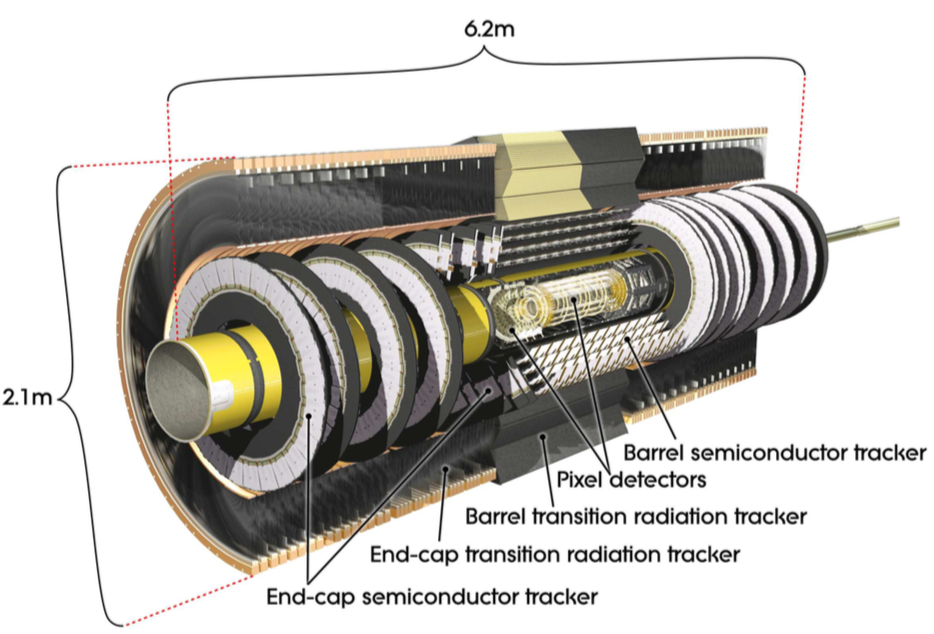
\includegraphics[width=0.75\textwidth]{figures/chapter2/inner_detector/atlas_inner_detector}
        \caption{
            Cross-sectional view of the ATLAS inner detector. Shown are the barrel
            and end-cap portions of the pixel, SCT, and TRT detectors.
        }
        \label{fig:atlas_inner_detector}
    \end{center}
\end{figure}

\begin{figure}[!htb]
    \begin{center}
        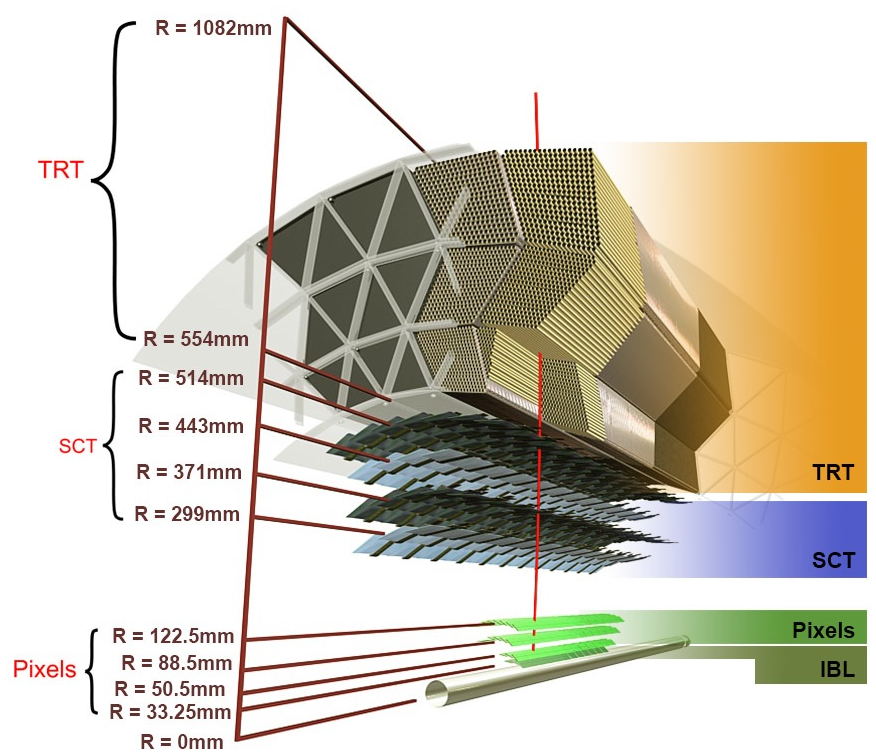
\includegraphics[width=0.7\textwidth]{figures/chapter2/inner_detector/atlas_ID_barrel_exploded}
        \raisebox{1.4cm}{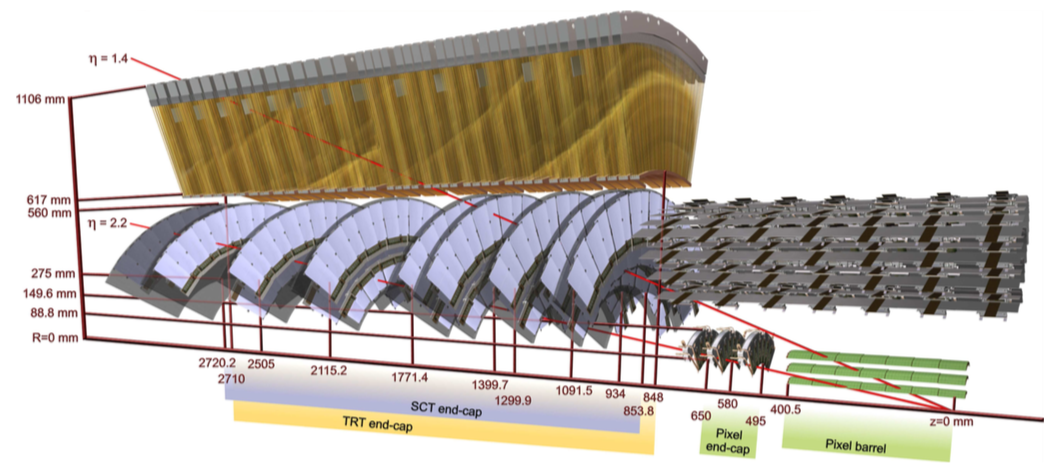
\includegraphics[width=0.95\textwidth]{figures/chapter2/inner_detector/endcap_ID_exploded}}
        \caption{
            Cut-away views of the barrel (\textit{top}) and end-cap (\textit{bottom}) portions
            of the ATLAS inner detector, with each of the three subdetectors indicated along with their
            envelopes in $r$ and in $z$.
        }
        \label{fig:atlas_ID_exploded}
    \end{center}
\end{figure}

\begin{figure}[!htb]
    \begin{center}
        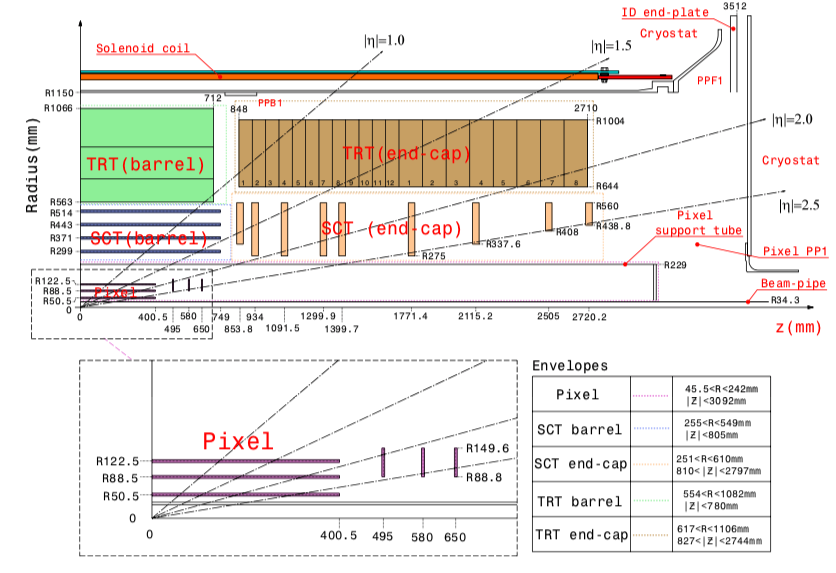
\includegraphics[width=0.9\textwidth]{figures/chapter2/inner_detector/atlas_ID_plan_view}
        \caption{
            Detailed drawing of the locations of the subsystems that make up the ATLAS ID.
            Positions in $r$, $z$, and $\eta$ are shown.
            From Ref.~\cite{ATLASCollab}.
        }
        \label{fig:atlas_ID_plan_view}
    \end{center}
\end{figure}

\subsubsection{The Pixel Detector and IBL}
\label{sec:id_pixel}

The pixel detector is the innermost subdetector of the ID, situated very near to and surrounding
the beam-pipe.
It is composed of three separate sections: a barrel section and two end-cap sections.
The barrel section  of the pixel detector has a cylindrical geometry and the end-cap sections
are disks centered on the beam-pipe.
The barrel section has four layers, each with increasing radius, and there are three disks in each
of the end-caps. This ID geometry, shown in Figure~\ref{fig:atlas_ID_exploded}, covers
the region $\lvert \eta \rvert < 2.5$.

The pixel detector, being so near the $pp$ collisions, is subject to the highest particle
fluxes of any other subsystem.
As a result, it is built to have very fine granularity: its sensing elements consist of
$250$\,\micron~thick detectors housing pixels of reverse-biased n-type silicon semiconductor material,
each having a nominal size of $50\times400\,\micron^2$.
In total, there are roughly 80 million channels read out from the pixel detector alone.
This allows for the pixel detector's fine spatial hit resolution of $10\,\micron$ in
$(r-\phi)$ and $115\,\micron$ along $z$.

The innermost layer of the pixel detector's barrel section is referred to as the
\textit{Insertable B-Layer} (IBL), and was installed at the beginning of the Run 2
data-taking period~\cite{Capeans:1291633}.
It corresponds, essentially, to the instrumentation of the ATLAS beam-pipe, as seen in Figure~\ref{fig:pixel_detector_trans},
and is located at a radial distance of 3.3\,cm.
It alone accounts for 8 million readout channels of
the pixel detector --- resulting in an ultra precise spatial hit resolution of $8\,\micron$ in $(r-\phi)$ and
$40\,\micron$ along $z$.
Beyond improving the overall measurements and reconstruction of charged particle tracks,
the IBL was installed in order to improve the performance of secondary vertex
reconstruction --- an essential ingredient to the algorithms associated with
the reconstruction and identification of jets originating from the decays
of $b$-hadrons whose decays occur at radial distances frequently beyond that
of the IBL, as illustrated in Figure~\ref{fig:bhadron_decay_length}..

\begin{figure}[!htb]
    \begin{center}
        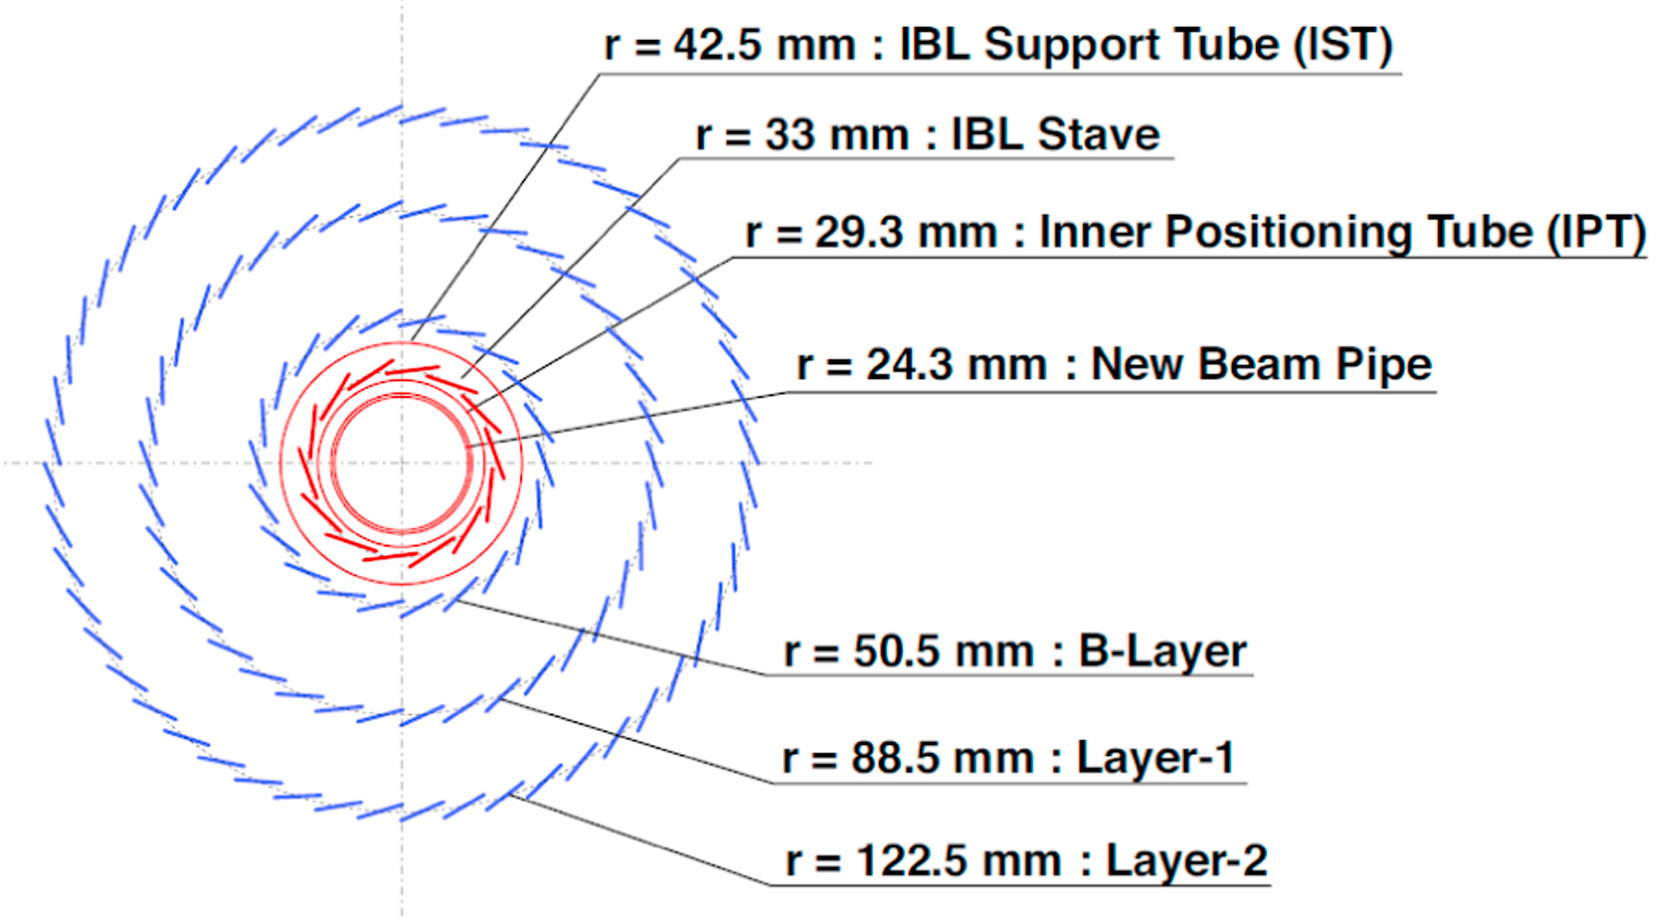
\includegraphics[width=0.8\textwidth]{figures/chapter2/inner_detector/pixel_detector_trans}
        \caption{
            Transverse view of the barrel section of the pixel detector, showing
            the innermost layer, the Insertable B-Layer (IBL), and its support structure (red) as well as the
            three surrounding layers (blue). From Ref.~\cite{Backhaus:2016ctq}.
        }
        \label{fig:pixel_detector_trans}
    \end{center}
\end{figure}

%\begin{figure}[!htb]
%    \begin{center}
%        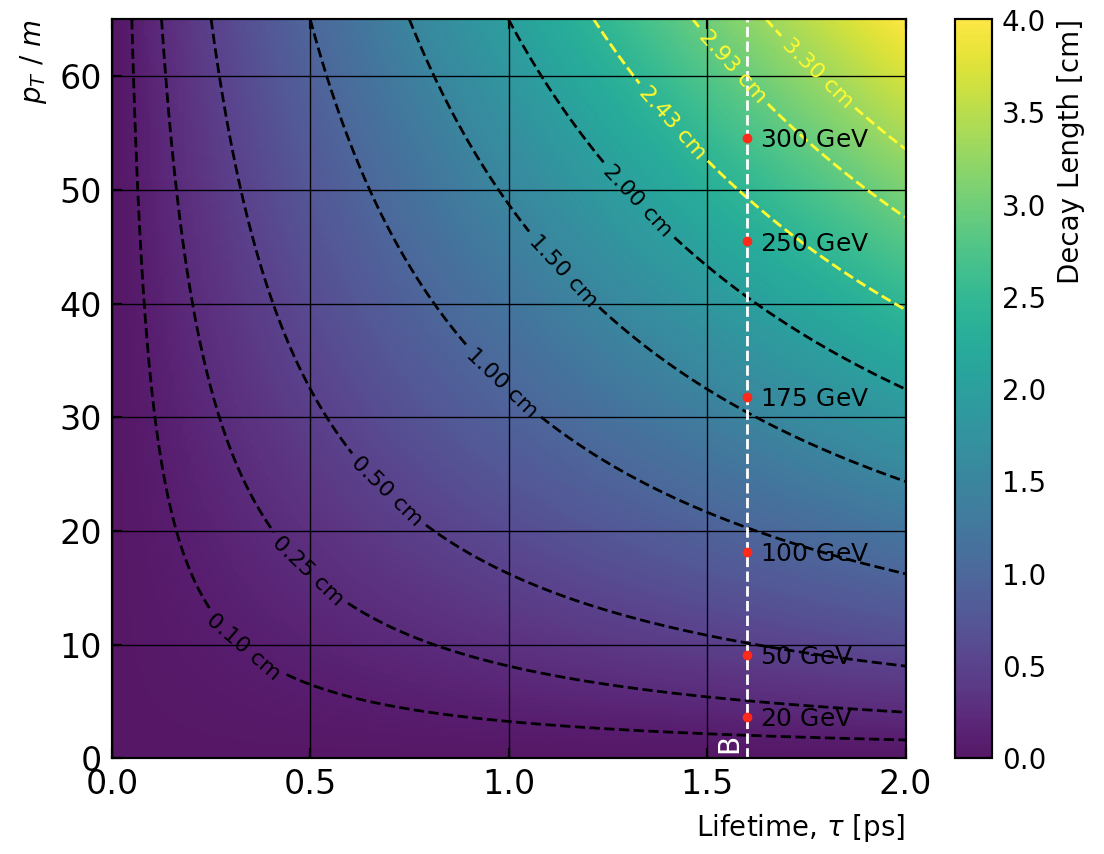
\includegraphics[width=0.7\textwidth]{figures/bhadron_decay_length_ibl}
%        \caption{
%            Particle decay length as a function of its lifetime and transverse momentum normalised
%            to its rest mass.
%            The white-dashed line indicates the average lifetime of $B$-hadron species, taken
%            as 1.6\,ps, with a mass taken to be 5.5\,GeV.
%            The red-dots along the $B$-hadron line indicate locations for specific transverse momenta
%            for the decaying $B$-hadron.
%            The yellow contours indicate the locations of the IBL (Figure~\ref{fig:pixel_detector_trans}),
%            with 2.43\,cm corresponding to the beam-pipe radius.
%            {\color{red}{Perhaps move this plot elsewhere?}}
%            {\color{red}{Add references to PDG}}
%        }
%        \label{fig:bhadron_decay_length}
%    \end{center}
%\end{figure}

\subsubsection{The Semiconductor Tracker}
\label{sec:id_sct}

The semiconductor tracker (SCT), like the pixel detector, uses silicon semiconductor-based sensing
elements.
It surrounds the pixel detector, as illustrated in Figure~\ref{fig:atlas_ID_exploded},
and has similar barrel and end-cap geometries.
The barrel section of the SCT is composed of 4 cylindrical layers and the end-caps consist
of 9 disks.
The silicon sensing elements are in a strip-like geometry with
$80\,\micron$ strip pitch.
The strips in the barrel section run parallel to the beam-pipe and those in the
end-caps are perpendicular, extending along the radial direction.\footnote{
The SCT layers in both the barrel and end-cap sections additionally contain small-angle (40\,mrad) stereo strips (c.f. Figure~\ref{fig:mm_stereo}) to allow for measurement of both
$(r-\phi)$ and $z$ information.}
The spatial hit resolution of the SCT is $17\,\micron$ in $(r-\phi)$ and $580\,\micron$
along $z$.
%At a given azimuthal ($\phi$) position, the barrel section two roughly 6\,cm long
%strips: each extending outwards from $z=0$ in the $\pm z$ direction.

\subsubsection{The Transition Radiation Tracker}
\label{sec:trt}

The outermost layer of the ATLAS ID, surrounding the SCT, is the transition
radiation tracker (TRT).
The TRT is a tracking volume designed around the proportional drift tube concept
and is composed of polyimide drift tubes (straws) that are 4\,mm in diameter.
The barrel section of the TRT conains up to 73 layers of 144\,cm-long straws aligned parallel to the
beam-pipe while the end-cap section has 160 straw planes composed of 37\,cm long straws arranged radially
into wheels (see Figure~\ref{fig:atlas_ID_exploded}).
Each straw of the TRT has a 31\,\micron~-width gold-coated wire at its center which acts as anode
and is grounded, while the inner walls of each straw are kept at a potential of
approximately $-1.5$\,kV.
A track hit in a given straw is the result of the 70\% Xe -- 27\% CO$_2$ -- 3\% O$_2$ gas mixture contained
in the straw volume being ionised and the resulting electrons (ions) drifting to
the center wire (inner wall) of the straw. The induced current from the drifting
charge is converted to an electrical signal and read out.

On average, a single charged-particle track leaves 36 hits in the TRT.
The TRT only provides $(r-\phi)$ information (no $z$ information),
for which it has a per-straw hit resolution of $130\,\micron$.
The relatively poor hit resolution, when compared to the silicon based
tracking detectors, is compensated by the large number of hits per track which
lead to very long measured track lengths as compared to the pixel and SCT detectors.
Additionally, the straws are embedded in and individually separated by
a polypropelene fiber which induces transition-radiation photons to be produced.
The amount and pattern of transition radiation depends on the mass of the passing
particle: the passage of an electron will produce significantly more transition radiation
than heavier charged particles, such as the copiously-produced pion.
Information provided by the TRT therefore provides additional discrimination
power between electrons and pions and enhances the performance of ATLAS' electron identification algorithms
that primarily depend on information coming from the calorimeter systems (Section~\ref{sec:calo_em}).
